\documentclass[11pt]{article}
\usepackage[left=0.5in,top=0.75in,right=0.5in,bottom=0.75in]{geometry}
\usepackage{amsthm,amsfonts,amssymb,float,graphicx,amsmath,siunitx,longtable,tabularx,enumitem,bm,caption,subcaption,multirow,stmaryrd,xcolor}
\usepackage[version=4]{mhchem}
\usepackage[section]{placeins}
\usepackage[version=4]{mhchem}

\input{../../Macros.tex}
\usepackage{hyperref}
\usepackage[url=false,style=ieee]{biblatex}
\addbibresource{../../Thesis Proposal/Proposal_bib.bib}
\AtEveryBibitem{\clearfield{month}}
\AtEveryBibitem{\clearfield{day}}

\newcommand{\vect}[1]{\underline{#1}}
\newcommand{\matr}[1]{\underline{\underline{#1}}}

\title{Ph.D. Project 1}

\author{Chris Womack}

\numberwithin{equation}{section}
\begin{document}

\maketitle

\begin{abstract}
Enjoy.
\end{abstract}

\clearpage

\section{Response Functions for Climate Emulation}

\subsection{Previous Work: JAMES Paper}

\textbf{A brief summary of our previous methodology. Given a general experiment:}
\begin{enumerate}
  \item Calculate an ERF profile for said experiment.
  \item Use LOWESS (or another algorithm) to smooth both ERF and temperature profiles; smoothing is applied at both the global and spatial levels.
  \item Calculate spatially explicit response functions via deconvolution of the smoothed profiles.
  \item Generate realistic ERF profiles (e.g. either from CMIP experiments or something like FaIR).
  \item Convolve the new ERF profiles with the response functions to predict spatially resolved temperatures.
\end{enumerate}
\textbf{Through this process, our JAMES paper shows a few key ideas:}
\begin{itemize}
  \item ERF is a skillful predictor variable for both spatial and global temperatures.
  \item Response functions are a skillful method to predict both spatial and global variables and can capture behavior that is impossible for pattern scaling to represent (e.g. the fishhook).
  \item Response functions allow for rapid emulation of large ensembles of policy-relevant climate scenarios.
  \item Deconvolution is a valid approach for diagnosing response functions.
\end{itemize}
\textbf{However, it is also limited in a few ways:}
\begin{itemize}
  \item As illustrated by Figure \ref{fig:responses}, the actual skill of the emulator is unfortunately heavily dependent on the skill of the smoothing algorithm, rather than the methodology itself; this figure shows that artificial smoothing is the only thing guaranteeing stability in response function diagnosis and that there's no one-size-fits-all smoothing (e.g. the smoothing parameter is manually tuned, so while the parameter works well for temperature, it reduces precipitation almost to pattern scaling, no time history). This robustness is the major issue!
  \item The smoothing also has the additional drawback of obfuscating how we would rigorously go about e.g. creating an inverse model for our emulator, incorporating stochastic terms, and accounting for aerosols (aerosol impacts are "spikes" in the ERF profile which are smoothed out almost entirely). Another way of saying this is that, it is unclear how we would apply useful relationships from statistical mechanics (we would like to leverage these in making an emulator for the sake of mathematical formalism) when smoothing has been applied to the system.
\end{itemize}
\textbf{Overall, we need to overcome these issues if we want our emulator to be more broadly applicable while still being mathematically rigorous.} A side effect of this pursuit is that we should also be able to improve the overall predictive skill of the emulator in the process of making these improvements.

\clearpage

\begin{figure}[ht]
  \begin{subfigure}{0.45\textwidth}
    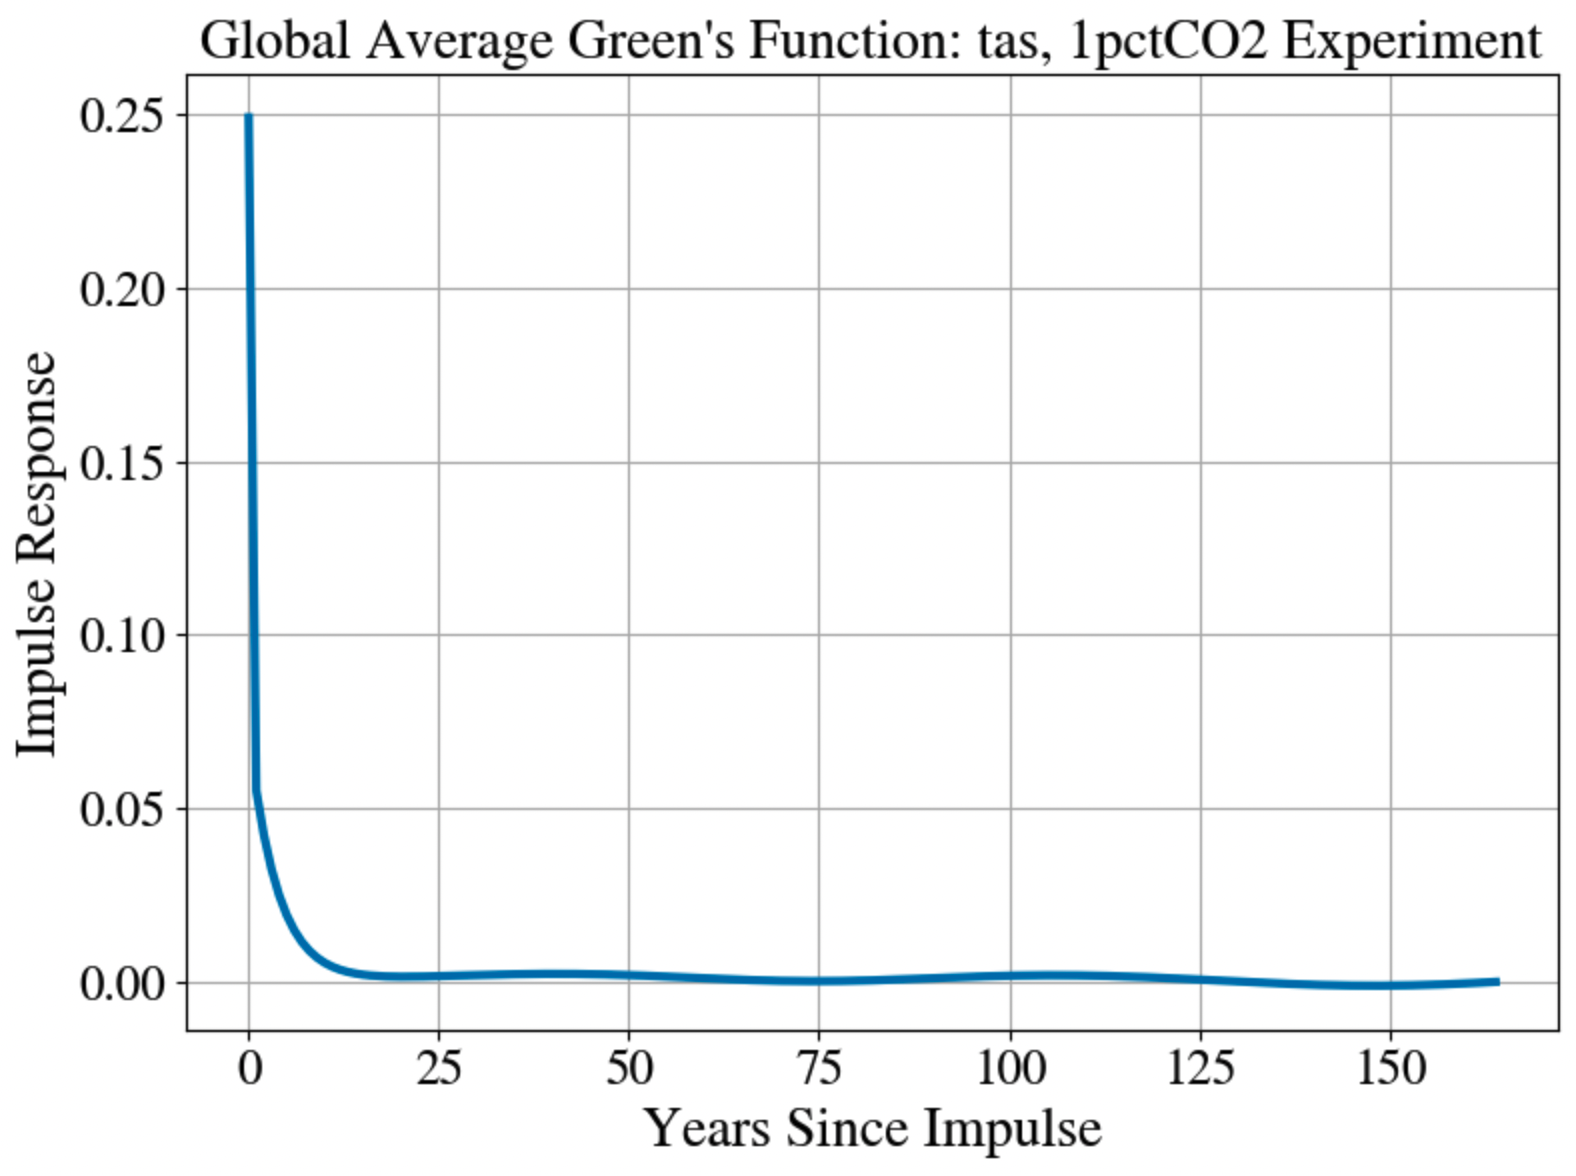
\includegraphics[width=\linewidth]{Figures/tas_1.png}
    \caption{\textit{1pctCO2} global temperature response function, high smoothing.} \label{fig:a}
  \end{subfigure}\hspace*{\fill}
  \begin{subfigure}{0.45\textwidth}
    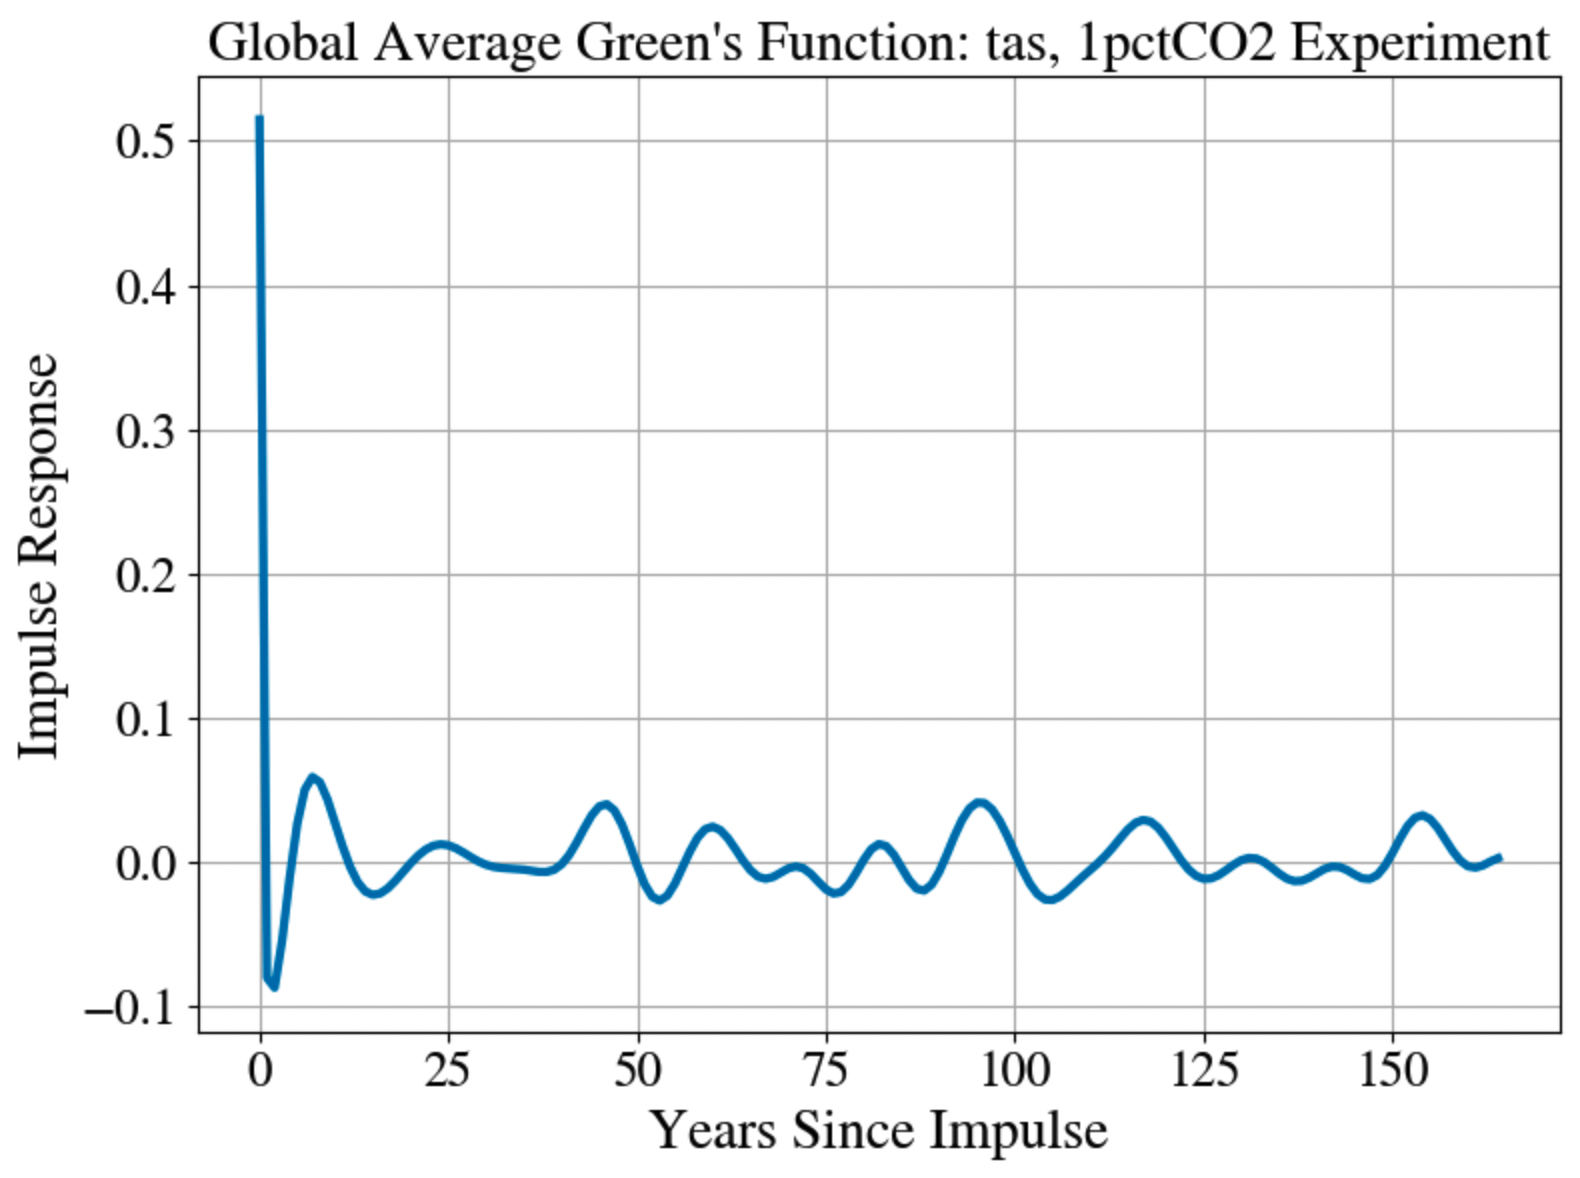
\includegraphics[width=\linewidth]{Figures/tas_2.png}
    \caption{\textit{1pctCO2} global temperature response function, low smoothing.} \label{fig:b}
  \end{subfigure}
  \medskip
  \begin{subfigure}{0.45\textwidth}
    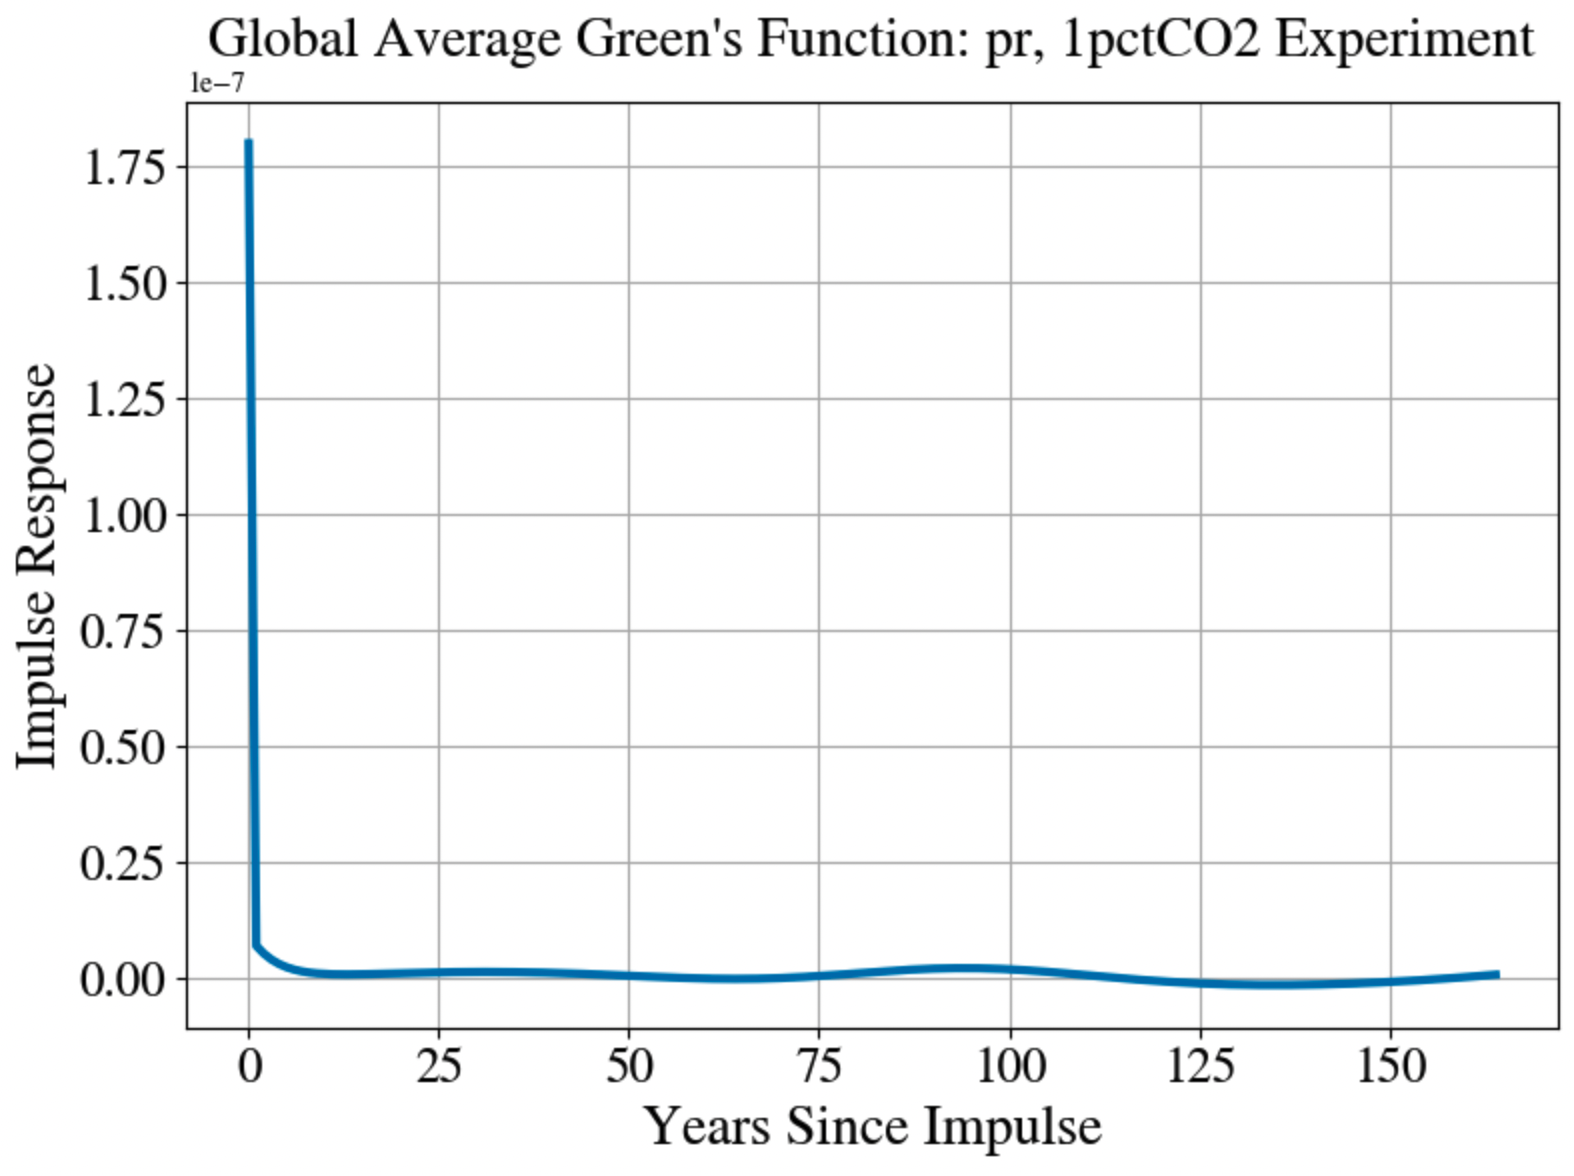
\includegraphics[width=\linewidth]{Figures/pr_1.png}
    \caption{\textit{1pctCO2} global precipitation response function, high smoothing.} \label{fig:c}
  \end{subfigure}\hspace*{\fill}
  \begin{subfigure}{0.45\textwidth}
    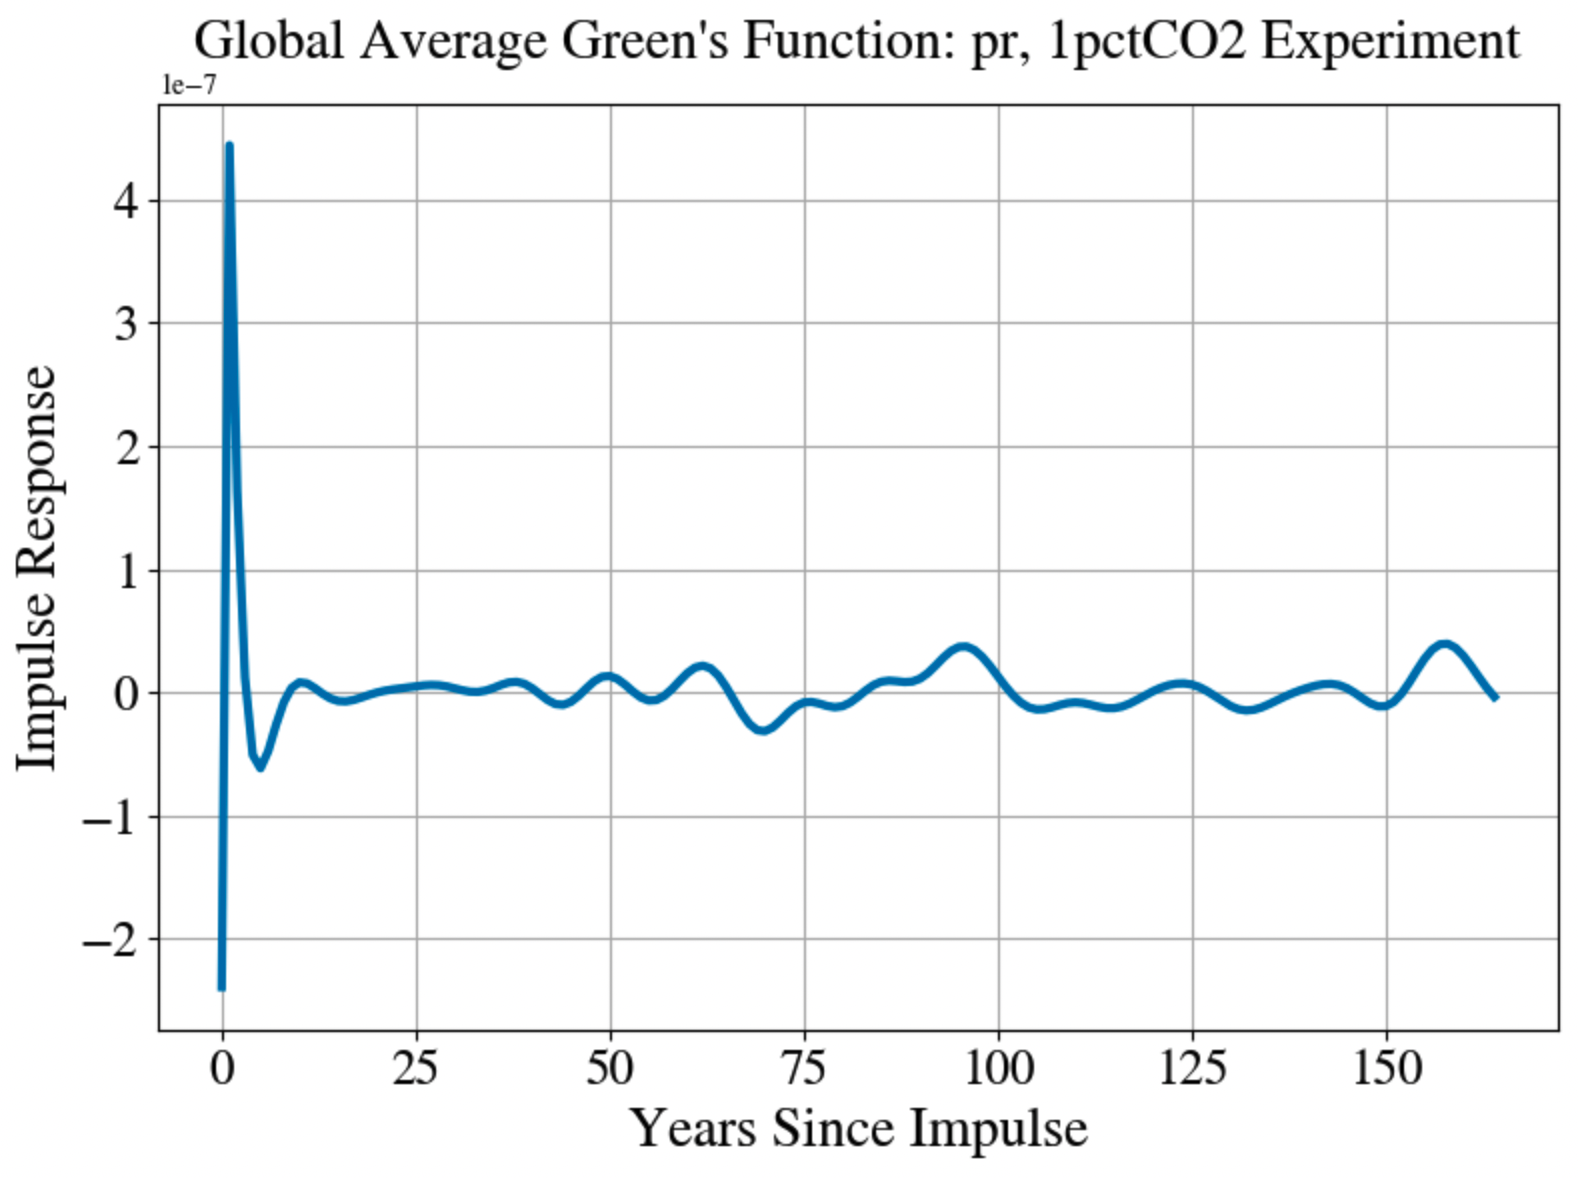
\includegraphics[width=\linewidth]{Figures/pr_2.png}
    \caption{\textit{1pctCO2} global precipitation response function, low smoothing.} \label{fig:d}
  \end{subfigure}
  \medskip
  \begin{subfigure}{0.45\textwidth}
    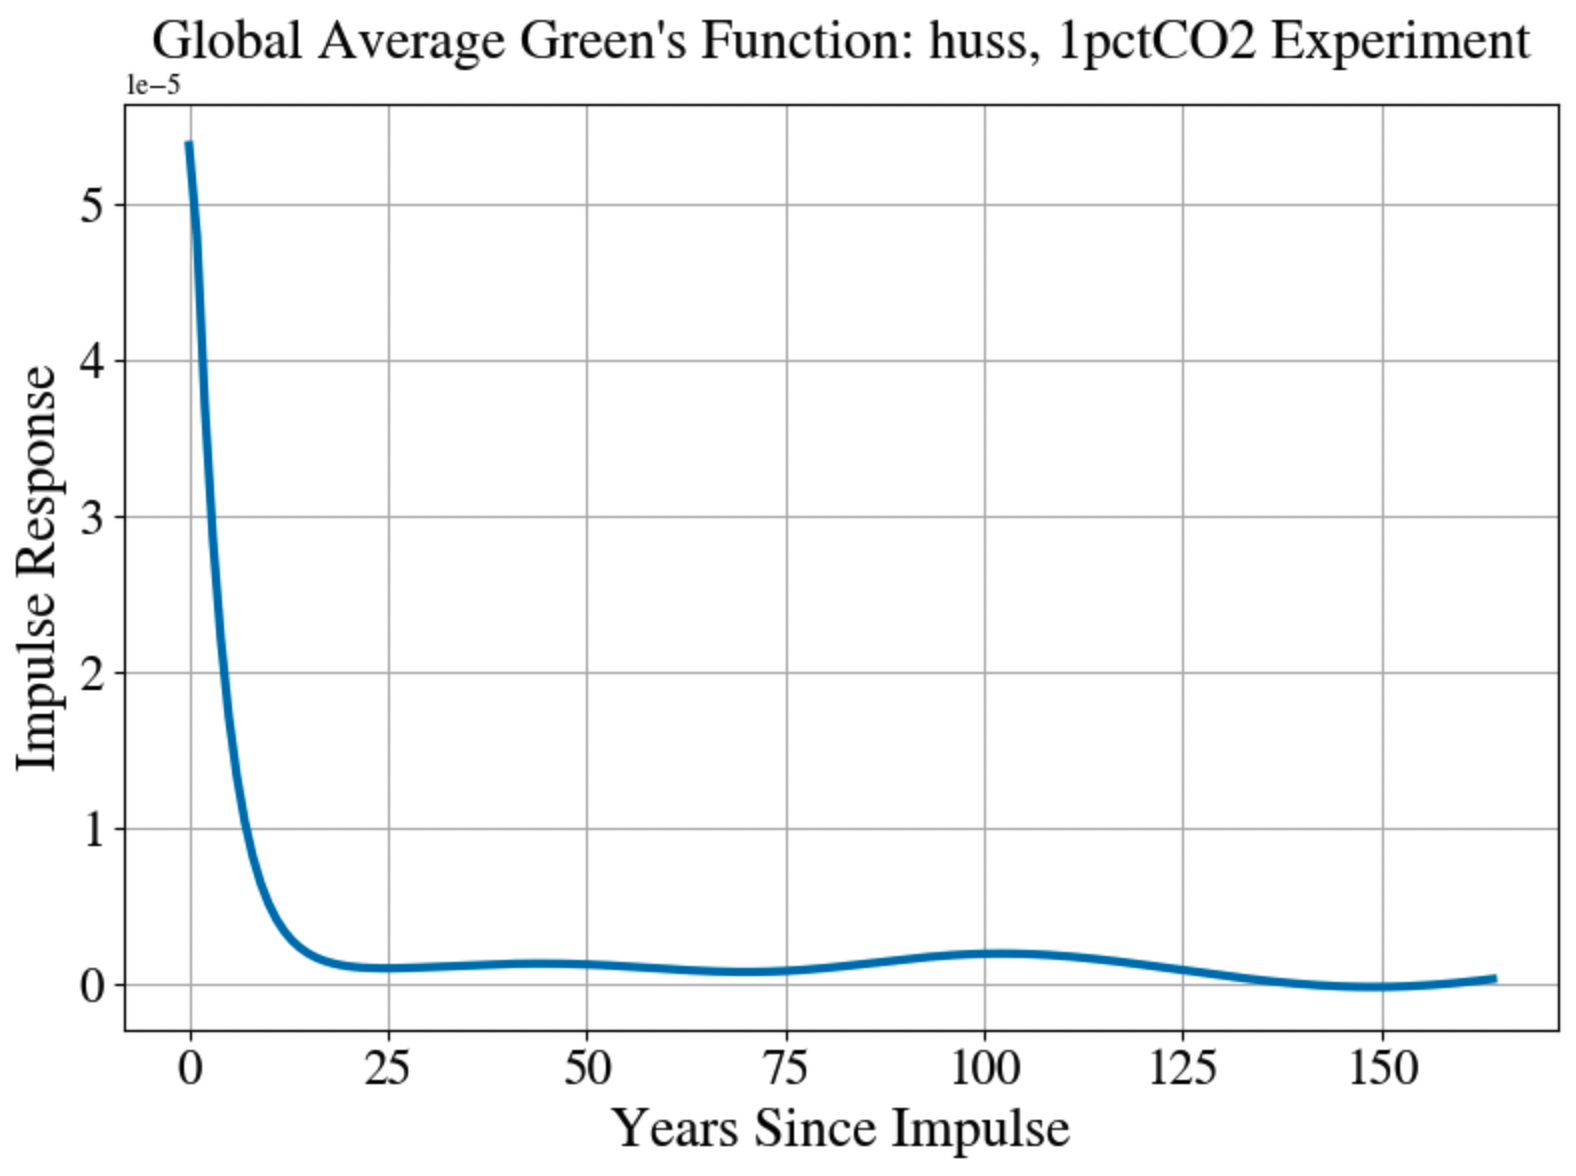
\includegraphics[width=\linewidth]{Figures/huss_1.png}
    \caption{\textit{1pctCO2} global relative humidity response function, high smoothing.} \label{fig:e}
  \end{subfigure}\hspace*{\fill}
  \begin{subfigure}{0.45\textwidth}
    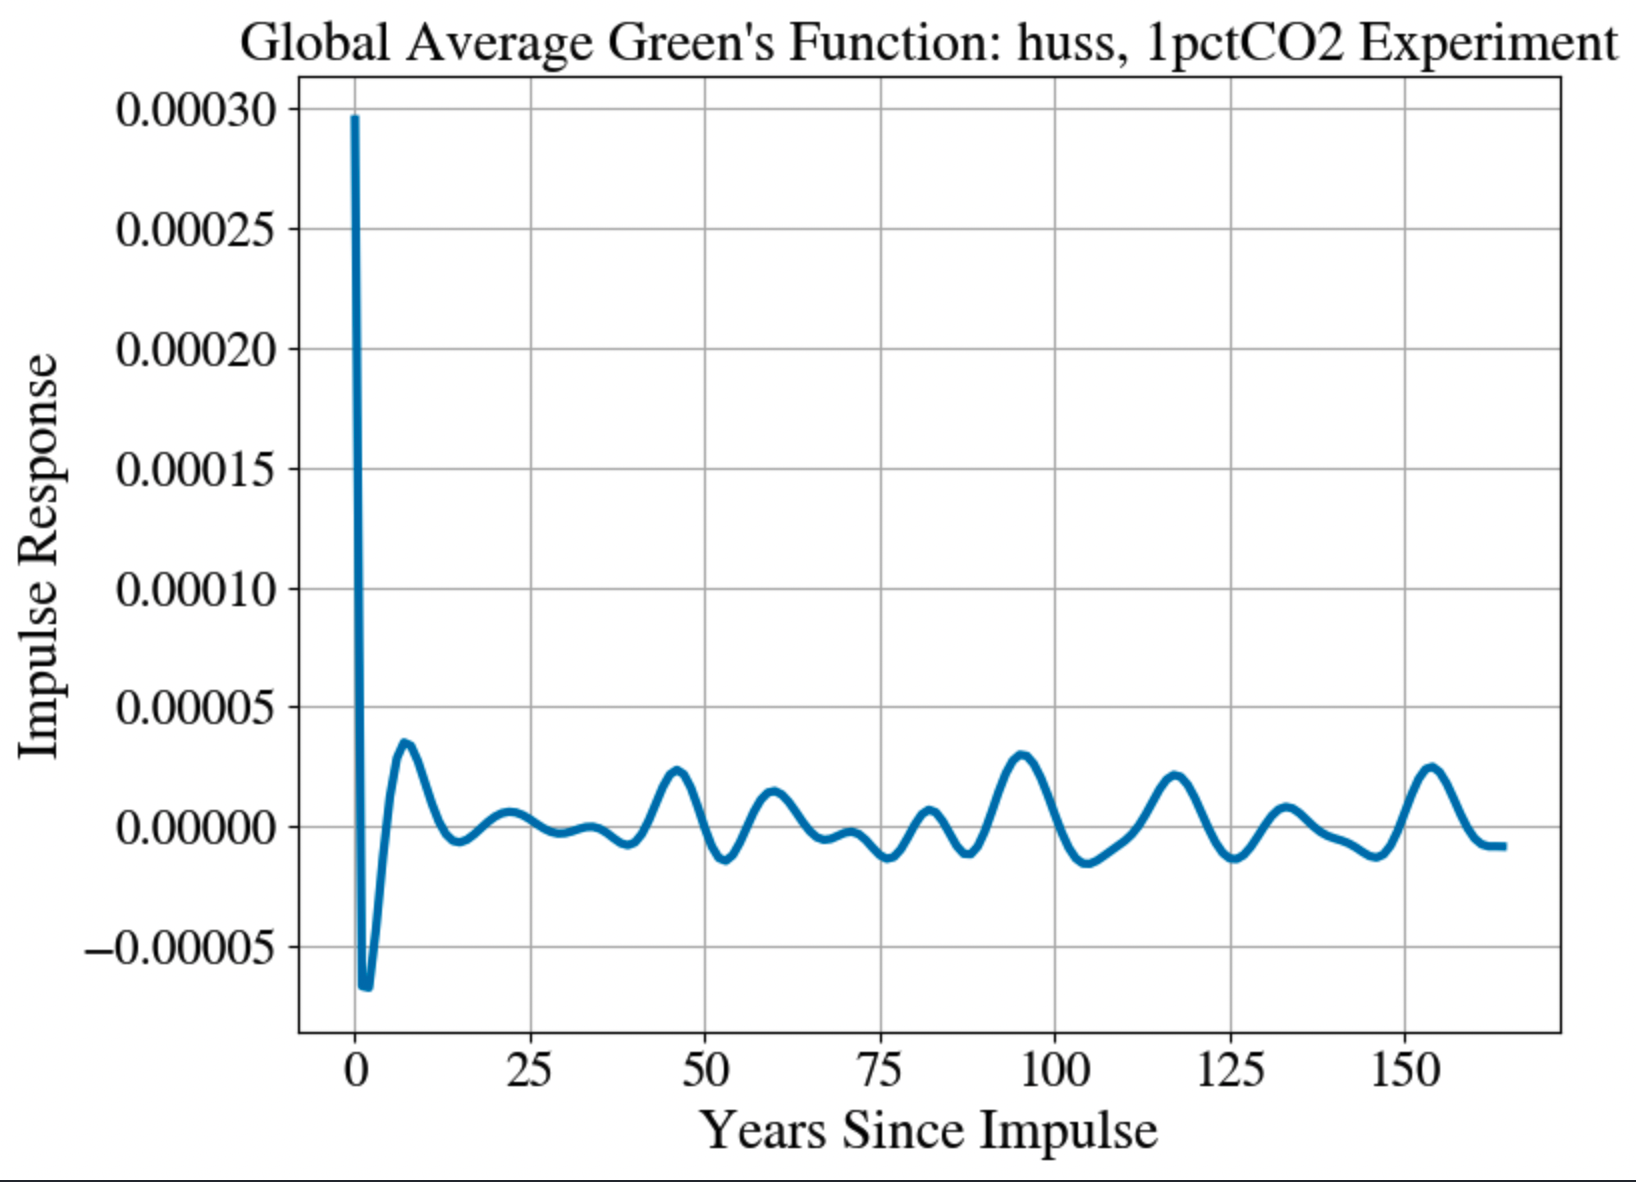
\includegraphics[width=\linewidth]{Figures/huss_2.png}
    \caption{\textit{1pctCO2} global relative humidity response function, low smoothing.} \label{fig:f}
  \end{subfigure}
  \caption{Global average response functions for temperature, precipitation, and relative humidity derived through deconvolution. Left and right columns denote high and low levels of smoothing, respectively.} \label{fig:responses}
  \end{figure}

  \clearpage

\subsection{Ongoing Theoretical Work: Response Functions}

In this section, I outline the work which I have been doing (primarily with Glenn) to create an alternate method to derive response functions - this method is meant to overcome the issues outlined in the previous section and improve overall accuracy. One high-level way to think about this method is that we are ultimately performing a deconvolution-like operation, but in terms of the spatial and temporal modes of the system rather than the raw data like the previous method.

\subsection*{Initial Assumptions}

Suppose we assume that temperature (or another climate variable of interest) can be represented by a linear differential equation. For simplicity, we are assuming linearity, stationarity (the statistics of the system are constant in time), and that there are no hidden variables (unknowns which we cannot measure and impact the system); these assumptions are also fundamental to methods such as pattern scaling, the success of which allows us to believe they are generally reasonable assumptions. This leaves us with the following relationship:
\begin{equation}\label{eq:lindiff}
  \PD{T(\mathbf{x},t)}{t} = L(\mathbf{x},\mathbf{x}')T(\mathbf{x}',t) + \gamma(\mathbf{x})F(t),
\end{equation}
which has variables:
\begin{itemize}
  \item $T(\mathbf{x},t)$: Spatially resolved temperature; units of $\left[\text{Kelvin}\right]$, dimension $(N_{\text{lat}} \times N_{\text{lon}}, N_t)$;
  \item $L(\mathbf{x},\mathbf{x}')$: Unknown linear operator, describes how the value of $T$ at a point $\mathbf{x}$ depends on the values of $T$ at other points, $\mathbf{x}'$; units of $\left[1/\text{time}\right]$, dimension $(N_{\text{lat}} \times N_{\text{lon}}, N_{\text{lat}} \times N_{\text{lon}})$;
  \item $\gamma(\mathbf{x})$: Spatial component of the forcing; units of $\left[\text{Kelvin}/\text{time} \times 1/\text{forcing}\right]$, dimension $(N_{\text{lat}} \times N_{\text{lon}}, 1)$;
  \item $F(t)$: Temporal component of the forcing; units of $\left[\text{forcing}\right]$, dimension $(1, N_t)$;
\end{itemize}
where the dimensions $N_{\text{lat}}, \, N_{\text{lon}}, \, \text{ and } N_t$ correspond to the number of latitude, longitude, and time points, respectively.

In the case of our original work, we considered $\gamma(\mathbf{x}) = o(\mathbf{x})$, where $o(\mathbf{x})$ is a vector of ones, i.e. no spatial dependence to the forcing, and used ERF as $F(t)$; this is not the only choice however, as we could consider a non-mixed forcing and include its spatial component (in theory, easily extendible to aerosols - in practice, there's likely data availability issues).

Our ultimate goal is to determine the unknown linear operator, or a surrogate for said operator, which will allow us to apply our initial relation to new systems of interest. E.g. deconvolution was one method to solve for this operator, which we could then convolve with new forcing profiles.

\subsubsection*{Dimensionality Reduction}

Before I begin with the actual methodologies for deriving response functions, I'll first present a simple dimensionality reduction technique. A fundamental part of this work moving forward is reducing the dimensionality to make the problem more compact; this has the potential cobenefits of allowing us to smooth via restricting the number of modes we keep, as well as allowing for some explainability in the dynamics (e.g. which modes represent ENSO?).

Using Equation \ref{eq:lindiff} directly in any capacity is likely computationally expensive when considering full climate models, as $N_{\text{lat}} \times N_{\text{lon}} \gg N_t$. Beginning from Equation \ref{eq:lindiff}, we instead use the SVD to separate our variable interest into its spatial and temporal modes:
\begin{equation}
  T(\mathbf{x},t) = g(\mathbf{x},m)\Sigma(m,n)V^T(n,t) = g(\mathbf{x},m)a(m,t),
\end{equation}
where $m = \min(|\mathbf{x}|,|t|)$. This can be completed using either EOFs or the SVD, I have chosen SVD here simply out of personal preference; Glenn has thoughts on which is better overall to use.

We can apply more sophisticated dimensionality reduction techniques if needed, but as of right now, I think that this simple decomposition gives us everything we need.

\subsubsection{Method 1: Direct derivation of Green's functions}

I'll begin from the most straightforward way to derive a response function. If you actually know/have access to the governing equation(s) for the system of interest, you can simply set $F(t) = \delta(t)$, which then gives you direct access to the Green's function. This can only be done once the system is in an equilibrium state though, not when the system is still transient (i.e. applying an impulse during the transient regime does not directly give the impulse response, but rather a potentially nonlinear combination of responses),
\begin{align}
  T(\mathbf{x},t)|_{F(t) = \delta(t)} = G(\mathbf{x},t).
\end{align}
This can also be done with the same dimensionality reduction techniques as above,
\begin{align}
  a(m,t)|_{F(t) = \delta(t)} = G(m,t).
\end{align}
This implicitly assumes we know the spatial structure of the forcing as well. We can then apply the response functions simply through convolution as,
\begin{align}
  T(\mathbf{x},t) &= \gamma(\mathbf{x}) \int_0^t d\tau \, G(\mathbf{x},t) F(t - \tau), \\
  a(m,t) &= \gamma(m) \int_0^t d\tau \, G(m,t) F(t - \tau), \quad \gamma(m) = g(m, \mathbf{x}) \gamma(\mathbf{x}).
\end{align}
In the second case, we have the additional step of actually calculating the temperature through $T(\mathbf{x},t) = g(\mathbf{x},m)a(m,t)$; again, this is still likely far more computationally efficient than working with the parent dataset.

This approach is what's used in much of the literature around response functions and linear response theory, especially those with a robust statistical mechanics approach (e.g. Lucarini, Lembo, and Ragone et al.). They generally use the step change \ce{CO2} experiments (e.g. \textit{2xCO2} or \textit{4xCO2}) and scale the response by the magnitude of the forcing.

Glenn has brought up the distinction between a Green's function and a response function is that, while a Green's function has a governing equation, a response function does not necessarily satisfy that equation. This approach is governed by Equation \ref{eq:lindiff}, but the next approach doesn't necessarily fulfill that requirement anymore.

\subsubsection{Method 2: Direct inference from the data}

Without access to the governing equations, things are a bit more tricky. When I'm referring to "access" to the governing equations, this can also be thought of as a violation of our main assumptions; e.g. we technically have access to the governing equations underlying any ESM, but temperature is no longer guaranteed to satisfy Equation \ref{eq:lindiff} - hence why we refer to these now as response functions.

We begin by rewriting Equation \ref{eq:lindiff} discretely, using a first-order forward difference,
\begin{align}
  \PD{T(\mathbf{x},t)}{t} \approx \frac{\Delta T(\mathbf{x},t)}{\Delta t} = \frac{[T(\mathbf{x},t + \Delta t) - T(\mathbf{x},t)]}{\Delta t},
\end{align}
where $\Delta t$ is the size of the timestep. We can then derive an expression for how to timestep $T(\mathbf{x},t)$ using the unknown operator:
\begin{align}
  \frac{\Delta T(\mathbf{x},t)}{\Delta t} &= L(\mathbf{x},\mathbf{x}')T(\mathbf{x}',t) + \gamma(\mathbf{x})F(t),\\
  T(\mathbf{x},t+\Delta t) &= \left(\Delta t \, L(\mathbf{x},\mathbf{x}') + \delta_{\mathbf{x},\mathbf{x}'}\right) T(\mathbf{x},t) + \Delta t \, \gamma(\mathbf{x})F(t)\label{eq:timestep}.
\end{align}
We then rearrange this system to solve for $L(\mathbf{x},\mathbf{x}')$:
\begin{align}
  L(\mathbf{x},\mathbf{x}') = \left[\frac{\Delta T(\mathbf{x},t)}{\Delta t} - \gamma(\mathbf{x})F(t)\right]T^+(t, \mathbf{x}')
\end{align}

If we instead want to first reduce the dimensionality of the system, we can rewrite Equation \ref{eq:lindiff} as,
\begin{align}
  g(\mathbf{x},m)\PD{a(m,t)}{t} &= L(\mathbf{x},\mathbf{x}')g(\mathbf{x}',m)a(m,t) + \gamma(\mathbf{x})F(t),\\
  \PD{a(m,t)}{t} &= g^{-1}(m,\mathbf{x})L(\mathbf{x},\mathbf{x}')g(\mathbf{x}',m)a(m,t) +\gamma(m)F(t),
\end{align}
where $\gamma(m) = g^{-1}(m,\mathbf{x})\gamma(\mathbf{x})$. Written discretely, this becomes,
\begin{align}
  \frac{\Delta a(m,t)}{\Delta t} &= g^{-1}(m,\mathbf{x})L(\mathbf{x},\mathbf{x}')g(\mathbf{x}',m)a(m,t) + \gamma(m)F(t),\\
  \frac{\Delta a(m,t)}{\Delta t}  &= N(m,m)a(m,t) + \gamma(m)F(t),
\end{align}
where $\Delta a(m,t)  = [a(m,t + \Delta t) - a(m,t)]$. We seek to solve for $N(m,m)$, and thus, $L(\mathbf{x},\mathbf{x}')$,

\begin{align}
  N(m,m) &= \left[\frac{\Delta a(m,t)}{\Delta t} - \gamma(m)F(t) \right]a^+(t,m),\\
  L(\mathbf{x},\mathbf{x}') &= g(\mathbf{x},m)N(m,m)g^{-1}(m,\mathbf{x}).
\end{align}
Given an initial condition and forcing, $L(\mathbf{x},\mathbf{x}')$ can then be used with Equation \ref{eq:timestep} to integrate forward in time. Summarizing, the process is as follows:
\begin{enumerate}
  \item Compute $T(\mathbf{x},t)$ from a general experiment.
  \item Decompose $T(\mathbf{x},t)$ into $g(\mathbf{x},m)a(m,t)$ using a modal decomposition, e.g. SVD.
  \item Calculate $\Delta a(m,t)$ using a finite difference scheme, e.g. $\Delta a(m,t) = [a(m,t + \Delta t) - a(m,t)]$.
  \item Calculate the pseudo-inverse of $a(m,t)$, such that $a(m,t)a^+(t,m) = 1$.
  \item Find the reduced order linear operator, $N(m,m) = \left[\frac{\Delta a(m,t)}{\Delta t} - \gamma(m)F(t) \right]a^+(t,m)$.
  \item Validate all eigenvalues of $N(m,m)$ are negative and have magnitude less than 1. If not, eliminate the problematic eigenvalues.
  \item Calculate the full-dimensional linear operator from the spatial modes: $L(\mathbf{x},\mathbf{x}') = g(\mathbf{x},m)N(m,m)g^{-1}(m,\mathbf{x})$.
  \item Given a forcing, $\gamma(\mathbf{x})F(t)$, and initial condition, $T(\mathbf{x},t_0)$, timestep our system using \ref{eq:timestep}.
\end{enumerate}
In theory, we can calculate $L(\mathbf{x},\mathbf{x}')$ from any experiment, provided we know the spatial and temporal components of the forcing. In practice, if the magnitude of the forcing is too large (or the transient response is dominant), it is likely to excite unstable modes in the system, leading to $L(\mathbf{x},\mathbf{x}')$ with enough unstable eigenvalues that we cannot accurately represent the system even if we throw those eigenvalues out; perturbation experiments are likely to perform better. Further testing is required to see if this will function for climate models, but I'll speculate that it's likely, given that the perturbations in the climate system are relatively small in magnitude.

\subsubsection{Method 3: Direct Deconvolution}

Now let's instead begin by assuming that temperature can be derived through convolution of the unknown response function, $R(\mathbf{x}, t)$, with the known forcing, $\gamma(\mathbf{x}) F(t)$:
\begin{align}
  T(\mathbf{x},t) = \gamma(\mathbf{x}) \int_0^t d\tau \, R(\mathbf{x},t) F(t - \tau).
\end{align}
In the ideal case where our forcing is an impulse, and we are directly solving a single ODE, $R(\mathbf{x},t) = G(\mathbf{x},t)$. I.e. the response function and the Green's function are identical. The response function in practice though comes from a full climate model with much greater complexity, and is not guaranteed to satisfy the original ODE in the way that $G(\mathbf{x},t)$ is.

We now discretize the above equation, rewrite in matrix form, and finally, rearrange to solve for $R(\mathbf{x},t)$
\begin{align}
  T(\mathbf{x},t_k) &= \Delta t \, \gamma(\mathbf{x}) \sum_{k = 0}^{N_t} R(\mathbf{x},t_k) F(t_{N_t - k}),\\
  \mathbf{T}(\mathbf{x}) &= \Delta t \, \gamma(\mathbf{x}) \mathbf{F} \mathbf{R}(\mathbf{x}),\\
  \mathbf{R}(\mathbf{x}) &= \frac{\mathbf{F}^{-1} \gamma^+(\mathbf{x}) \mathbf{T}(\mathbf{x})}{\Delta t}.
\end{align}
This should look familiar, as it's the same methodology from our JAMES paper, with the additional tweaks that: 1. the forcing is allowed to vary spatially and 2. we allow for a timestep which isn't $\Delta t = 1$; this does still assume the size of the timestep is constant. For completeness, this process can also be done with dimensionality reduction:
\begin{align}
  a(m,t) &= \gamma(m) \int_0^t d\tau \, R(m,t) F(t - \tau),\\
  \mathbf{R}(m) &= \frac{\mathbf{F}^{-1} \gamma^+(m) \mathbf{a}(m)}{\Delta t}.
\end{align}

Deconvolution as a whole however, has a big issue which is more readily apparent in frequency space. Using a Fourier transform, our convolution becomes,
\begin{align}
  \mathcal{F}\left[T(\mathbf{x},t)\right] &= \gamma(\mathbf{x}) \mathcal{F}\left[ \int_0^t d\tau \, R(\mathbf{x},t) F(t - \tau)\right] \\
  T(\mathbf{x},\omega) &= \gamma(\mathbf{x}) R(\mathbf{x},\omega) F(\omega).
\end{align}
I.e., in frequency space, convolution becomes multiplication. Thus, our deconvolution becomes division,
\begin{align}
  R(\mathbf{x},\omega) &= \frac{T(\mathbf{x},\omega)}{\gamma(\mathbf{x}) F(\omega)},\\
  R(\mathbf{x},t) &= \frac{1}{\gamma(\mathbf{x})}\mathcal{F}^{-1}\left[\frac{T(\mathbf{x},\omega)}{ F(\omega)}\right].
\end{align}
Therefore, if we have any zeros or large differences in magnitude between the smallest and largest frequencies, our system is clearly unstable. This issue is what causes the need for artificial smoothing in the original deconvolution methodology.

There are some potential ways around this issue, as deconvolution is a commonly encountered and well-studied problem in signal processing; it can also be thought of as a Fredholm integral equation of the first kind, which is also a well-studied problem. Another way may be to add a simple regularization term. Casting this problem as a least squares problem, we can add a regularization term,

\begin{align}
  ||\mathbf{F}\mathbf{R}(\mathbf{x}) - \mathbf{T}(\mathbf{x})||^2 + \alpha ||\mathbf{R}(\mathbf{x})||^2,
\end{align}
where we choose the norm depending on what type of regularization we want to apply (e.g. ridge vs. lasso). I tried some variations on this and didn't have a huge amount of luck, though I think I could definitely be more rigorous and try again.

\subsubsection*{Aside: Relation between Methods 2 and 3 (have Glenn check this)}

Methods 2 and 3 are actually quite closely related. If we start from Equation \ref{eq:lindiff} and integrate in time, we get,
\begin{align}
  \PD{T(\mathbf{x},t)}{t} &= L(\mathbf{x},\mathbf{x}')T(\mathbf{x}',t) + \gamma(\mathbf{x})F(t),\\
  T(\mathbf{x},t) &= \int_0^t d\tau \, \exp(L(\mathbf{x},\mathbf{x}')(t-\tau)) \gamma(\mathbf{x})F(t).
\end{align}
Comparing this to the convolution definition, we see that,
\begin{align}
  T(\mathbf{x},t) &= \gamma(\mathbf{x}) \int_0^t d\tau \, R(\mathbf{x},t - \tau) F(t).\\
  R(\mathbf{x},t) &= \exp(L(\mathbf{x},\mathbf{x}')t) \gamma(\mathbf{x}').
\end{align}
In words, both of these methods are deconvolutions of sorts, but at different steps in the process. I.e. method 2 assumes that the linear operator is going to satisfy the original ODE, but the same restrictions (e.g. temperature being differentiable) do not exist for the response function.

The eigenvalues of the linear operator, $L(\mathbf{x},\mathbf{x}')$, dictate the decay rate for the response function, while the spatial pattern of the forcing determines the amplitude of the functions. Another way of interpreting this in light of the previous instability argument is that the instability occurs when the eigenvalues of the system are either non-negative or have a magnitude greater than 1.

\subsubsection{Method 4: Assume G can be represented using only a few timescales}

The final methodology I'll outline here again begins from the governing equation. This time, however, we note that the Green's function satisfies this equation with the assumption of an impulse forcing,
\begin{align}
  \PD{G(\mathbf{x},t)}{t} = L(\mathbf{x},\mathbf{x}') G(\mathbf{x}',t) + \gamma(\mathbf{x}) \delta(t - \tau).
\end{align}
Solving this equation yields,
\begin{align}
  G(\mathbf{x},t) = e^{\tau L(\mathbf{x},\mathbf{x}')} \gamma(\mathbf{x}').
\end{align}
Thus, our Green's function is an exponentially decaying function. Suppose now we only consider a few of the leading order modes to be significant, leading to the approximation,
\begin{align}
  e^{\tau L(\mathbf{x},\mathbf{x}')} &\approx h_j(\mathbf{x}) e^{-\tau \lambda_j} h_j^+(\mathbf{x}'),\\
  G(\mathbf{x},t) &\approx h_j(\mathbf{x}) e^{-\tau \lambda_j} h_j^+(\mathbf{x}')\gamma(\mathbf{x}'),
\end{align}
where $h_j(\mathbf{x})$ and $\lambda_j$ are used to approximate the unknown linear operator, and $h_j^+(\mathbf{x}')$ is the pseudo-inverse of $h_j(\mathbf{x})$ (if we keep e.g., 4 modes, $4 \ll N_{\text{lat}} \times N_{\text{lon}}$). Implicit in this description is that we will be summing over all $j$ indices. Therefore, calculating our Green's function becomes a nonlinear fitting exercise given by,
\begin{align}
  \tilde{T}(\mathbf{x},t,h_j(\mathbf{x}),\lambda_j) &= h_j(\mathbf{x}) \left[ \int_0^t d\tau \, e^{-\tau \lambda_j} F(t - \tau) \right] h_j^+(\mathbf{x}') \gamma(\mathbf{x}'),\\
  \argmin_{h_j(\mathbf{x}), \, \lambda_j} &||T(\mathbf{x},t) - \tilde{T}(\mathbf{x},t,h_j(\mathbf{x}),\lambda_j)||^2_2.
\end{align}
For completeness, we can also do this using a modal decomposition,
\begin{align}
  \PD{G(m,t)}{t} &= L(m,n) G(n,t) + \gamma(m) \delta(t - \tau),\\
  G(m,t) &= e^{\tau L(m,n)} \gamma(n),\\
  e^{\tau L(m,n)} &\approx h_j(m) e^{-\tau \lambda_j} h_j^+(n),\\
  G(m,t) &\approx h_j(m) e^{-\tau \lambda_j} h_j^+(n)\gamma(n),\\
  \tilde{a}(m,t,h_j(m),\lambda_j) &= h_j(m) \left[ \int_0^t d\tau \, e^{-\tau \lambda_j} F(t - \tau) \right] h_j^+(n) \gamma(n),\\
  \argmin_{h_j(m), \, \lambda_j} &||a(m,t) - \tilde{a}(m,t,h_j(m),\lambda_j)||^2_2.
\end{align}
With the same caveat that we will need to reconstruct our temperature from our modal estimation after the fact.

\subsection{Now let's get random}
\subsubsection{A very simple way to capture noise}
If we instead treat the governing equation as stochastic, we get,
\begin{align}
  \PD{T(\mathbf{x},t,j)}{t} = L(\mathbf{x},\mathbf{x}')T(\mathbf{x}',t,j) + \gamma(\mathbf{x})F(t) + \beta(\mathbf{x})\zeta(t,j),
\end{align}
where $j$ denotes an ensemble member, and $\beta(\mathbf{x})\zeta(t,j)$ represent the spatial and temporal modes of the stochastic component of the forcing. Denoting $\overline{T}(\mathbf{x},t)$ as the ensemble mean, we recover the original formulation,
\begin{align}
  \PD{\overline{T}(\mathbf{x},t)}{t} = L(\mathbf{x},\mathbf{x}')\overline{T}(\mathbf{x}',t) + \gamma(\mathbf{x})F(t).
\end{align}
For completeness, we can also write the stochastic formulation using a modal decomposition,
\begin{align}
  \PD{a(m,t,j)}{t} = L(m,n)a(n,t,j) + \gamma(m)F(t) + \beta(m)\zeta(t,j).
\end{align}
We will continue in modal space for the rest of this section. We would first solve for the mean component using any of the formulations in the previous section, which then allows to solve for the stochastic component for each ensemble member, 
\begin{align}
  \PD{\overline{a}(m,t,j)}{t} &= L(m,n)\overline{a}(n,t,j) + \gamma(m)F(t), \\
  \PD{a(m,t,j)}{t} - \PD{\overline{a}(m,t,j)}{t} &= \beta(m)\zeta(t,j).
\end{align}
There is a bit of subtlety we have to keep track of here though, as our modal decomposition is now dependent on the ensemble member: $T(\mathbf{x},t,j) = g(\mathbf{x},m,j)a(m,t,j)$. This isn't a big deal, we just have to keep track of this.

The key issue I see with this methodology is that it doesn't actually get you a probability distribution to sample from. It treats the variability within each ensemble member as fixed. E.g. if you derive a "noise ensemble" using this process, and then perform inference by applying that noise to a new mean component (new meaning that it comes from a novel forcing profile), the new ensemble will have the \textit{exact same noise pattern as the original}. This isn't ideal, as we'd like to represent the distribution and take new samples from that.

One simple way around this is to use the statistics from the noise ensemble to rebuild the underlying probability distribution, but this is subject to a few pitfalls: e.g. you're likely making a Gaussian assumption which may or may not be correct (like in Mengze's case, where the profile isn't Gaussian), and you'll be potentially missing the tail of the distribution - though I suppose this is the case for any data driven method, if it's not in the training data we simply won't see it.

\subsubsection{How about GPs?}

Another method (fairly new to me) is to lay a Gaussian Process (GP) prior over the problem of interest. For my own sake, a function, $f(t)$, is a GP if "any finite collection of its evaluations has a joint multivariate normal distribution" (thanks Shahine). A GP is fully determined by its mean and covariance functions,
\begin{align}
  f(t) &\sim \text{GP}(m,k),\\
  m(t) = \text{E}[f(t)], &\quad k(t,t') = \text{Cov}(f(t),f(t')).
\end{align}
I'm not sure what the exact formulation would look like, but one could imagine using (in a similar vein to Shahine's work) a deterministic forcing function, with a covariance function acting over past forcing trajectories with a \textit{spatial dependence} to that covariance function. It's definitely worth starting to test this sort of setup on simple problems to see how well it could capture that spatial pattern. I'll need help figure out the exact formulation for this though.

My main concern with this idea at the moment: how well would this perform on other variables of interest? Many might not have Gaussian distributions. Shahine suggested potentially setting up a transform such that,
\begin{align}
  g(\mathbf{x},t) &\sim \text{GP}(\mathbf{x},m,k), \\
  R(\mathbf{x},t) &= \psi(g(\mathbf{x},t)).
\end{align}
I.e. we still get to take advantage of the Gaussian assumption for some aspects of the problem, but we can end up with a non-Gaussian probability distribution after the transform. This won't have the same analytic properties as the pure GP, but could be a potential fix. We can also look into connecting Mengze's work to this impulse response function framework.

I'll need to dig much more into everything in this section!

\clearpage

\section{Paper 3 - Methods: Emulating the impact of spatially resolved forcings in climate models}\label{sec:paper3}

Almost an extension to paper 1 rather than its own full-contained system; i.e. it will probably build off a lot of the same mathematics. Frame this both in terms of climate impacts of spatially resolved forcings, but also considering the implications for e.g. air quality which is also poorly represented. I see this more as a GRL paper (whereas the previous two would be JAMES-esque), i.e. it's a short addendum which covers this specific contribution as something to highlight independently of the full emulator.

\subsection{Introduction}

\begin{itemize}
  \item Most climate emulators can't handle spatially resolved forcings (especially pattern scaling, though include references to forcing-specific patterns)
  \item I believe there are some purely ML references we could include here, but these are limited in their utility due to the explainability issue
\end{itemize}

\begin{itemize}
  \item Gap: ability to emulate the impact of spatially resolved forcings
  \item Solution: extension to methodology in paper 1 which allows for those effects to be tabulated
\end{itemize}

\subsection{Methods}

\begin{itemize}
  \item Extension of math from the previous section to include spatially resolved forcings
  \item Outline plan for how we would train/test this emulator along with whether it would fit into the aforementioned adjoint frameworks; inclusion of RAMIP data
  \item Roadmap how this contribution fits into the framework established by Anthony + Paolo for developing an "all-in-one" emulator which can go from emissions to AQ and climate outcomes
\end{itemize}

\subsection{Progress and Future Work}

\begin{itemize}
  \item Answers the important technical/methodological question of "how" we go about doing this in a rigorous way to lay the groundwork for other groups to improve on the method
  \item Increases utility of the emulator significantly by allowing regions to specify their own emissions scenarios and understand their local impacts, rather than being limited to the global emissions of others
  \item Similar to the last point, extremely pertinent to policymakers in regions with high aerosol emissions, as they can see how changing those emissions will impact their regions
\end{itemize}

\subsection{Collaborators}

\begin{itemize}
  \item Glenn Flierl - methods, math
  \item Paolo Giani - methods, concepts
  \item Anthony Wong - methods, concepts
  \item Arlene Fiori - concepts
  \item Noelle Selin - methods, concepts
  \item David Darmofal? - methods, math
\end{itemize}

\subsection{Data Availability}

\printbibliography

\end{document}